
\subsection{Heated backward-facing step}\label{ssec:HeatedBackwardFacingStep}
\begin{figure}[tb]
	\begin{center}
		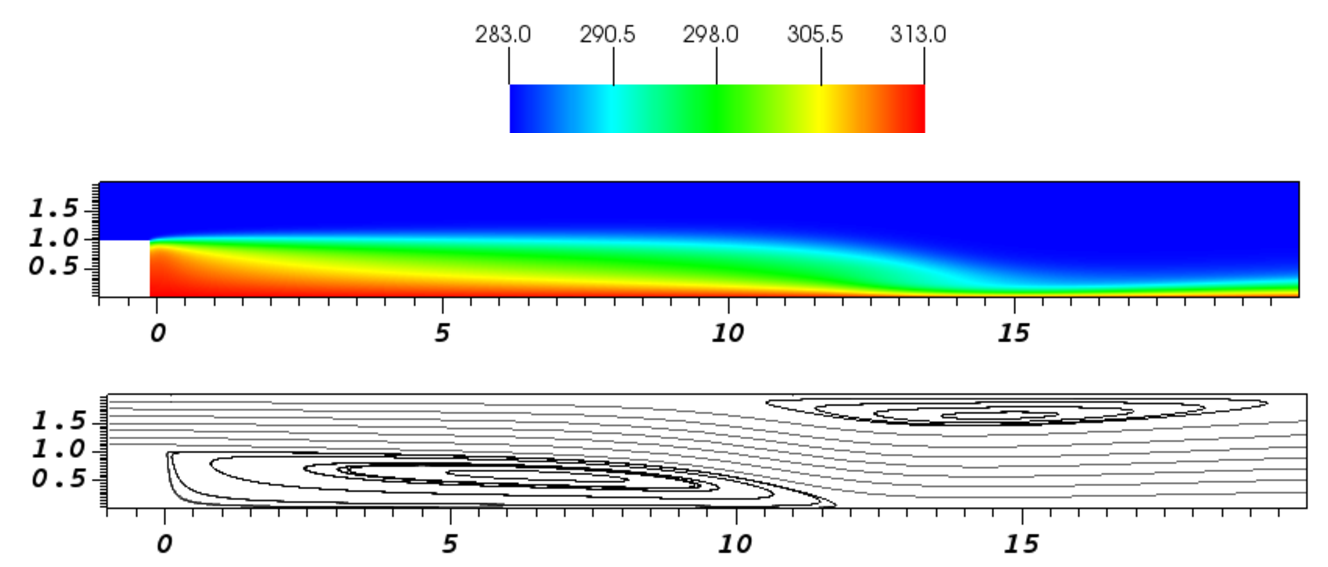
\includegraphics[width=\linewidth]{../plots/HBFS_TemperatureRe700_2.pdf}
		\caption{Temperature profile (top) and streamlines (bottom) corresponding to the backward-facing Step configuration for $\gls{Reynolds} = 400$ and an expansion ratio of two.}
		\label{BFS_Streamlines}
	\end{center}
\end{figure}

As an extension to the previous case, we seek to reproduce the results presented by \cite{xieFluidFlowHeat2016}, where the same backward-facing step configuration as presented in \cref{ssec:BackwardFacingStep} is studied, but with the particularity that in this case the bottom wall is heated to a constant temperature higher than the inlet temperature, thus featuring a non-isothermal system. The fluid entering the system has a temperature equal to $\hat T_0 = \SI{283}{\kelvin}$ and the bottom wall is set to a constant temperature of $\hat T_1 =\SI{313}{\kelvin}$
In the work of \cite{xieFluidFlowHeat2016} results are reported for the local Nusselt numbers and local friction coefficients $f_d$  along the bottom wall ($y = 0$) for different expansion ratios and Reynolds numbers. By putting together the definition of the Nusselt number ( $\gls{Nusselt} = \frac{\gls{HeatTransCoef}\hat{L}}{\gls{HeatConductivity}}$), Newton's law of cooling ($\hat{\vec{q}} = \hat{h} (\hat{T}_0 - \hat{T}_W )$), and Fourier's law of heat conduction ($\hat{\vec{q}} = \hat \lambda \hat{\nabla} \glsHat{temp}$) a expression for the local Nusselt number is obtained.
\begin{equation}
	\gls{NusseltLoc} = \frac{\hat L}{\hat T_0-\hat T_W}\hat \nabla \hat T \cdot \hat {\vec{n}}
\end{equation}
where $\hat L$ is a reference length. We choose $ \hat L = \hat S$ to be consistent with the definition of the Reynolds number of the reference. Furthermore, recognizing that the wall shear stress along the bottom wall $\tau_{\text{w}} = -\mu \nabla u \cdot \vec{n}$, the local friction factor can be written as
\begin{equation}
	f_d = \frac{8\nu} { (U_{\text{mean}})^2}  \nabla u \cdot \vec{n}
\end{equation}
It should be noted that for the range of temperature differences involved in this case, the variation of physical parameters such as density, viscosity, and thermal conductivity with respect to temperature has no appreciable influence on the calculated flow fields.

Simulations were conducted for different Reynolds numbers and expansion ratios. In \cref{BFS_Streamlines} the temperature field and streamlines corresponding to a calculation with $\gls{Reynolds} = 700$ are shown. Here, the apparition of the secondary vortex is seen in the top wall.

It must be noted here that the results obtained by us are substantially different from those reported by \cite{xieFluidFlowHeat2016}, and will not be shown here. However, in the work of \cite{henninkLowMachNumberFlow2022} the same is also noted, saying that with his method it was not possible to reproduce the results presented by \cite{xieFluidFlowHeat2016}. Comparing our results with those of Hennink we can observe that the same results are obtained. as demonstrated in \cref{fig:fd_Nu_plot}.% We can conclude from these results that the solver is able to deal with non-isothermal flows adequately.

\begin{figure}[tb]
	\pgfplotsset{
		group/xticklabels at=edge bottom,
		legend style = {
				at ={ (0.59,1.0), anchor= north east}
			},
		unit code/.code={\si{#1}}
	}
	\inputtikz{fd_Nu_plot1}
	\inputtikz{fd_Nu_plot2}
	\caption{Local friction factor and local Nusselt number along the bottom wall for $\gls{Reynolds} = 700$ and an expansion ratio of two. The solid lines corresponds to our solution and the marks to the reference \citep{henninkLowMachNumberFlow2022}}
	\label{fig:fd_Nu_plot}
\end{figure}



\FloatBarrier
